\section{Estudo da Cultura Organizacional segundo o Modelo Ogbonna \& Harris}
\qquad O Modelo Ogbonna \& Harris estuda a relação entre as variáveis de Estilos de liderança, Cultura organizacional e Performance organizacional. Este modelo foi derivado de um estudo empírico na Inglaterra através de os procedimentos científicos e estatísticos sobre a analise dos dados obtidos por questionários às empresas envolvidas.
%%%%%%%%%%%%%%%%%%%%%%%%%%%%%%%%%%%%%%%%%%%%%%%%%%%%%%%%%%%%%%%%%%%%%%%%%%%%%%%%%
\subsection{Modelo Ogbonna \& Harris}
\quad {\bf As variáveis  descritas de seguida, são as que foram consideradas no estudo.}
\emptyline
\begin{minipage}[t]{.31\linewidth}
\quad Estilos de Liderança:
\begin{itemize}
\setlength\itemsep{-0.3em}
\item Participativo
\item Orientado as pessoas\\
(Liderança de suporte)
\item Orientado as tarefas\\
(Liderança Instrumental\\ ou Diretiva\\ ou Transacional)
\end{itemize}
\end{minipage}
\begin{minipage}[t]{.31\linewidth}
\quad Tipos de Cultura:
\begin{itemize}
\setlength\itemsep{-0.3em}
\item Inovadora
\item Competitiva
\item Burocrática
\item Comunitária
\end{itemize}
\end{minipage}
\begin{minipage}[t]{.31\linewidth}
\quad Medição do Sucesso:
\begin{itemize}
\setlength\itemsep{-0.3em}
\item Satisfação dos Clientes
\item Taxa crescimento vendas
\item Cotação no mercado
\item Vantagens Competitivas
\item Volume de vendas
\end{itemize}
\end{minipage}
\minipagespace{.5cm}
Os resultados obtidos na determinação do estilo de liderança e tipo de cultura organizacional das empresas estudadas, e o modelo que foi criado são apresentados de seguida:
\begin{figure}[H]
\centering
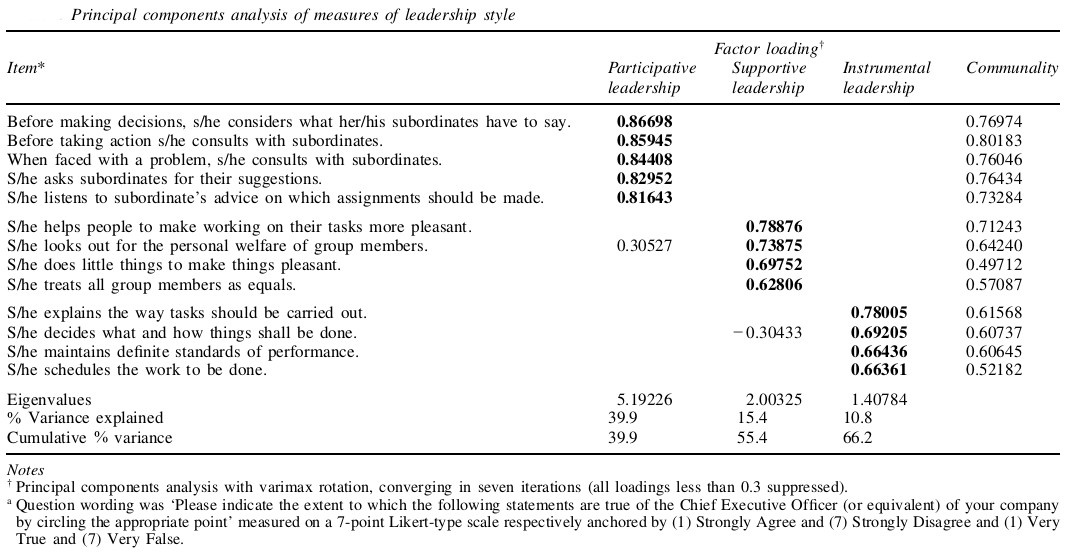
\includegraphics[scale=.4]{./image/OB/Leadership.jpg}\\
\caption{Inquérito do Estilos de Liderança \cite{article_1}}
\end{figure}\par
%%%%%%%%%%%%%%%%%%%%%%%%%%%%%%%%%%%%%%%%%%%%%%%%%%%%%%%%%%%%%%%%%%%%%%%%%%%%%%%%%
A tabela acima é o inquérito com os resultados das 322 companhias que serviram de amostras. Os resultados depois foram tratados por um método estatístico de forma a obter o modelo. Os estilos de liderança depois são determinado através do peso das questões que caraterizam cada uma.
%%%%%%%%%%%%%%%%%%%%
\begin{figure}[H]
\centering
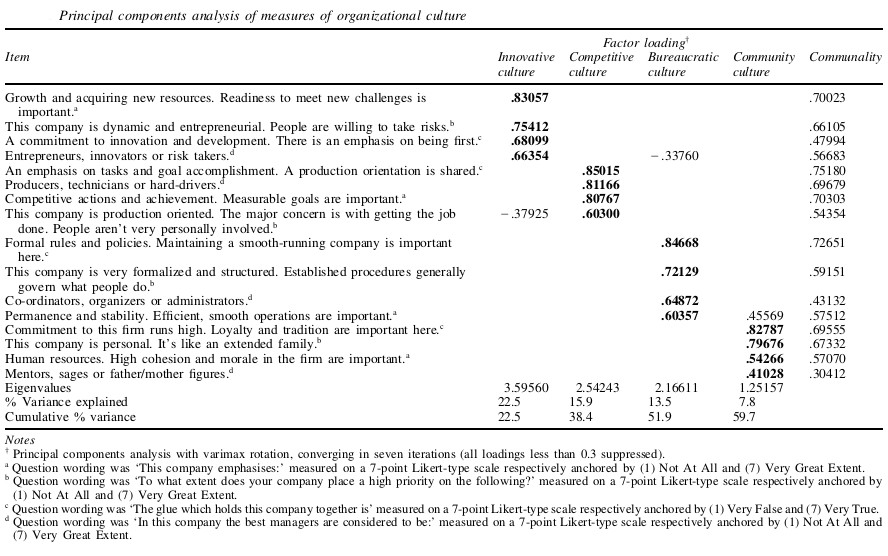
\includegraphics[scale=.5]{./image/OB/Culture.jpg}\\
\caption{Inquérito do tipo de Cultura Organizacional \cite{article_1}}
\end{figure}\par
%%%%%%%%%%%%%%%%%%%%
A tabela acima, demonstra as questões e os tipos de cultura que representam, em conjunto com a tabela do estilo de liderança e o tratamento dos dados Ogbonna \& Harris obterem o seu modelo.
%%%%%%%%%%%%%%%%%%%%
\begin{figure}[H]
\centering
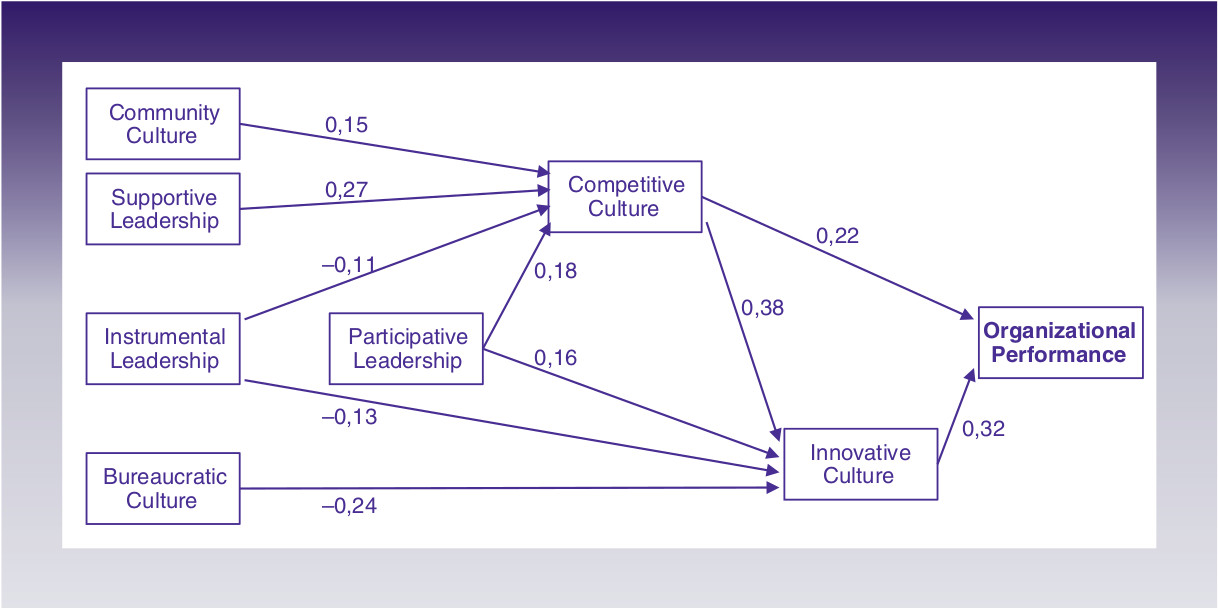
\includegraphics[scale=.35]{./image/OB/Ogbonna_Harris.jpg}\\
\caption{Modelo Ogbonna \& Harris \cite{article_1}}
\label{Modelo}
\end{figure}
Neste estudo foi observado que a relação entre o estilo de liderança e o sucesso não era tão bem percebido como a relação entre a de cultura organizacional e o sucesso. Descobriram que a cultura organizacional servia de mediador entre o estilo de liderança e o sucesso. O estilo de liderança não tinha influencia direta no seu sucesso mas indiretamente. Descobriram também que organizações com o tipo de cultura inovadora e competitiva eram mais bem sucedidas do que as companhias com cultura organizacional burocráticas ou comunitárias. A cultura inovadora e competitiva era mais focada para o exterior (posicionamento e resposta), e a cultura burocrática e comunitária para o interior (integração, coesão, uniformidade). As companhias com culturas burocráticas e comunitárias demonstravam uma relação insignificante e indireta entre cultura organizacional e sucesso, no entanto para as culturas inovadoras e competitivas existia uma forte e positiva relação. Enquanto, a cultura inovadora e competitiva preenchia quase 25 \% da variância na performance das organizações (sucesso), também se observou que apenas o tipo de liderança participativa e orientada às pessoas tinham uma correlação positiva com as culturas inovadoras e competitivas.
\emptyline
Concluindo que, as organizações com culturas inovadoras e competitivas, tendo um estilo de liderança orientada às pessoas e participativa seriam mais promissoras para melhorar o desempenho da organização e que devem focar-se em \textcolor{blue}{mudar} para uma cultura orientada para o exterior. \cite{article_1}
%%%%%%%%%%%%%%%%%%%%%%%%%%%%%%%%%%%%%%%%%%%%%%%%%%%%%%%%%%%%%%%%%%%%%%%%%%%%%%%%%
\subsection{Modelo Aplicado a S.Roque}
O Inquérito (\textit{igual figura 6}) abaixo é usado para medir os componentes principais para determinar a Cultura Organizacional.
\begin{table}[H]
\begin{adjustbox}{max width=\textwidth}
\begin{tabular}{ |c|l|c| }
\hline
\rowcolor[gray]{0.5}
Nº & Inquérito & \makecell[l]{Resp \\ 1 \; - \; 7} \\
\hline
1. & \makecell[l]{A organização preocupa-se com o crescimento e a aquisição de novos recursos, \\ e procura responder a novos desafios.} & \\
\hline
2. & \makecell[l]{A organização é dinâmica e empreendedora. \\ As pessoas estão dispostas a correr riscos.} & \\
\hline
3. & \makecell[l]{Existe um elevado empenho na inovação e no desenvolvimento. \\ Procuramos ser os primeiros.} & \\
\hline
4. & \makecell[l]{Consideram-se os melhores gestores os que são empreendedores, \\ Inovadores e tomadores de riscos.} & \\
\hline
5. & Existe uma elevada ênfase nas tarefas e no alcance de objetivos. & \\
\hline
6. & Considera-se que os melhores gestores são produtores e técnicos. & \\
\hline
7. & \makecell[l]{A organização valoriza as ações competitivas, \\ o sucesso e o alcance de objetivos mensuráveis.} & \\
\hline
8. & \makecell[l]{A organização é orientada para a produção. \\ Uma das maiores preocupações é fazer o que tem que ser feito. \\ Os empregados não estão muito envolvidos do ponto de vista pessoal.} & \\
\hline
9. & A organização valoriza muito as regras e as políticas formais. & \\
\hline
10. & \makecell[l]{A organização é muito formalizada e estruturada. \\ Os procedimentos estabelecidos orientam o que as pessoas devem fazer.} & \\
\hline
11. & Os melhores gestores são considerados os que são coordenadores ou organizadores. & \\
\hline
12. & Na organização valoriza-se a permanência, a estabilidade e a eficiência. & \\
\hline
13. & Valoriza-se muito a lealdade, a tradição e o empenhamento na organização. & \\
\hline
14. & A organização é uma espécie de grande família. & \\
\hline
15. & Valoriza-se muito a coesão e os recursos humanos. & \\
\hline
16. & \makecell[l]{Considera-se que os melhores gestores são os que atuam como mentores, \\ sábios ou figuras paternais/maternais.} & \\
\hline
\end{tabular}
\end{adjustbox}
\end{table}
{\tiny 1- A afirmação não se aplica rigorosamente nada à minha organização, 2- Não se aplica, 3- Aplica-se muito pouco, 4- Aplica-se alguma coisa,\\ 5- Aplica-se bastante, 6- Aplica-se muito, 7- A afirmação aplica-se completamente à minha organização
}
%%%%%%%%%%%%%%%%%%%%%%%%%%%%%%%%%%%%%%%%%%%%%%%%%%%%%%%%%%%%%%%%%%%%%%%%%%%%%%%%%
\begin{table}[H]
{\small
\begin{tabular}{|l|c|c|}
\hline
                                                                                                    & Média do Inquerito & \begin{tabular}[c]{@{}l@{}}Ogbonna \& Harris\\ (2000)\end{tabular} \\ \hline
\cellcolor[HTML]{C0C0C0}\begin{tabular}[c]{@{}l@{}}Cultura de inovação\\ {[}1-4{]}\end{tabular}     & 5,4 & 4,6 \cellcolor[HTML]{EFEFEF}                                           \\ \hline
\cellcolor[HTML]{C0C0C0}\begin{tabular}[c]{@{}l@{}}Cultura de Competição\\ {[}5-8{]}\end{tabular}   & 5,3 & 4,2 \cellcolor[HTML]{EFEFEF}                                           \\ \hline
\cellcolor[HTML]{C0C0C0}\begin{tabular}[c]{@{}l@{}}Cultura Burocrática\\ {[}9-12{]}\end{tabular}    & 4,7  & 4,3 \cellcolor[HTML]{EFEFEF}                                           \\ \hline
\cellcolor[HTML]{C0C0C0}\begin{tabular}[c]{@{}l@{}}Cultura de Comunidade\\ {[}13-16{]}\end{tabular} & 5  & 4,6 \cellcolor[HTML]{EFEFEF}                                           \\ \hline
\end{tabular}
}
\end{table}
%%%%%%%%%%%%%%%%%%%%%%%%
{\footnotesize
\textbf{Contribuições para o Inquérito:}\\
\textbf{-} \; \textcolor{green}{Paulo Campos} ; \quad \textcolor{green}{Daniel Carvalho} ; \quad \textcolor{green}{Bruno Pereira} ; \quad \textcolor{green}{Sérgio Santos}
}
%%%%%%%%%%%%%%%%%%%%%%%%%%%%%%%%%%%%%%%%%%%%%%%%%%%%%%%%%%%%%%%%%%%%%%%%%%%%%%%%%
